
\begin{abstract}

\end{abstract}
\section{Introduction}
Internet privacy, also commonly referred to as online privacy, is a subset of data privacy and a fundamental human right. We consider privacy to revolve around control, use and disclosure of one’s personally identifiable information.
However, our increasingly technologically-driven world puts great pressure on privacy. 
This is why several actors in the space are continuesly developinng different solutions to achieve anonymous communication and thus leveraging internet privacy.


\subsection{State of the art}
\subsubsection{Privacy protocols}
Tor is an open-source software for enabling anonymous communication. It is based on onion routing which encapsulates messages in layers of encryption and transmits them through a series of network nodes called onion routers. Tor however is susceptible to end-to-end correlation attacks conducted by an adversary who can eavesdrop the communication channels.These attacks reveal a wide range of information like the identity of the communicating peers.
Another project based on onion routing is I2P peer-to-peer network. I2P has different design choices from those of Tor:
\begin{itemize}
    \item Packet switched instead of circuit switched: routers maintain multiple tunnels per destination which increases significantly the scalability from $O(N)$ to $O(1)$ and resilience against failures.
    \item Unidirectional instead of bidirectional tunnels: which makes deanonymization harder but needs two sets of peers to be profiled since it's unidirectional.
    \item Peer profiles instead of directory authorities: I2P’s network information is stored in a DHT (information in the DHT is inherently untrusted) while Tor’s relay network is managed by a set of nine Directory Authorities.

\end{itemize}
I2P are vulnerable to eclipse attacks since no I2P router has a full view of the global network (similar to other peer-to-peer networks) and they also protect against only local adversaries (like Tor) and thus vulnerable to timing, intersection and traffic analysis attacks. I2P have also showed to be vulnerable to sybil and predecessor attacks inspite of the different contermeasures implemented to defeat them.
\\~\\Another existing solution for network privacy is VPN(Virtual Private Network). 
VPNs builds an encrypted tunnel between the client and server to transfer communication in a secure way and they also provide a new IP address (the one of the proxy) to help bypass censership and geolocalization blocks.
Due to the centralized trust model VPNs has, they suffer from inherent weaknesses like being a single point of failure. They are also vulnerable to powerful network eavedropers who can track the routed network traffic.
\\Those privacy concerns have motivated the creation of a new model of VPNs, dVPNs (Decentralized Virtual Private Networks) with no central authority and backed by blockchain technology. Orchid, Sentinel and Mysterium are the most known projects in the blockchain ecosystem providing dVPN solutions. These projects however are still vulnerable to end-to-end correlation attacks. 
\\~\\Mixnets are overlay networks of mix nodes that routes messages anonymously similarly to Tor.What differentiates mixnets from Tor is that mixnets are designed to provide metadata protection from global network adversaries by using cover traffic. Because mixnets add extra latency to network traffic, they are better-suited to applications that are not as sensitive to increased latency, such as messaging or email applications while applications like real-time video streaming are better suited for Tor. 
\\~\\First mixnet paper in 1981 by David Chaum didn't use any cover traffic and instead used a cascade topology which consists of stages connected in a fixed, sequential order where inputs are shuffled and transfered. This method however was not scalable and susceptible to traffic and active attacks. Since then, research has evolved to provide solutions with low latency while still providing high anonymity.
\\ One of the well known projects is Loopix. Loopix leverages cover traffic to resist traffic analysis while still achieving low- to mid-latency. To this end Loopix employs a mixing strategy that we call a Poisson Mix that is based on the independent delaying of messages, which makes the timings of packets unlinkable.
\\~\\ The goal of each one of these projects is to acheive low latency, low bandwidth overhead and strong anonymity or as we call it the anonymity trilemma. We present in the following a comparison table (from the Loopix paper) between different anonymous communication systems.

\begin{figure}[H]
    \centering
    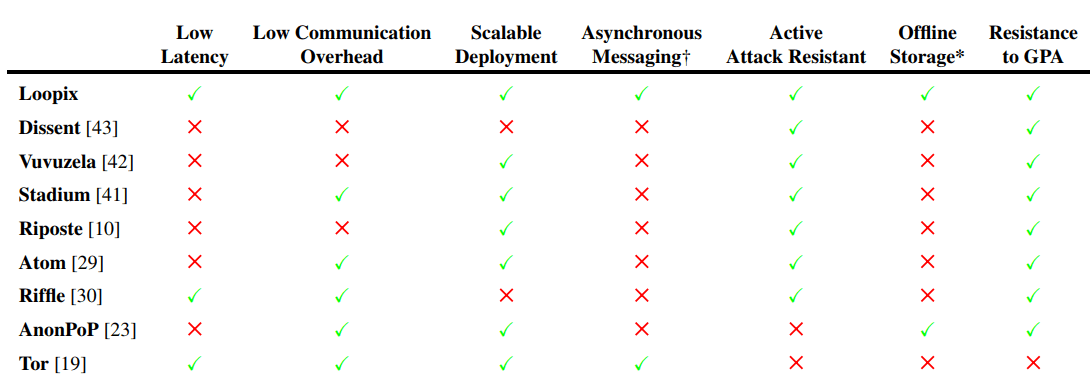
\includegraphics[width=11cm,height=11cm,keepaspectratio]{../whitepaper/images/state-of-the-art.png}
    \caption{Comparison between anonymous communication systems}
    \label{fig:Comparison between anonymous communication systems}
\end{figure}


\subsubsection{Scalability Layer 2 protocols}
Blockchain technology (mostly public blockchains like Bitcoin and Ethereum) suffers from two major issues: privacy and scalability. The latter is due to the fact that every node in the network needs to process every transaction, validate it and stores a copy of the entire state. The number of transactions Ethereum can process for example cannot exceed that of a single node which is currently 15 transactions per second.
\\~\\There have been multiple solutions proposed to treat the scalability issue such as sharding and off-chain computation. Both of these solutions intend to create a second layer of computation in order to reduce the load on the blockchain mainnet.
\\Off chain solutions like Plasma, Truebit and state channels process transactions outside the Blockchain while still guaranteeing a sufficient level of security and finality. State channels are better known as "payment channels". In models like the "Lightning Network", a payment channel is opened between two parties by committing a funding transaction, followed by making any number of transactions that update the channel's funds without broadcasting those to the blockchain, then closing the channel by broadcasting the final version of the settlement transaction.
\subsection{The HOPR vision}
HOPR is a decentralized incentivized mixnet that leverages privacy by design protocols. HOPR aims to protect people's metadata privacy and give them the freedom to use internet services safely and privately. HOPR runs on top of the Ethereum blockchain and uses three mechanisms to ensure users privacy via incentivisation: sphinx paquet format, proof-of-relay and probabilistic payments.




 




